\section{Zielsetzung}
In diesem Versuch sollen Magnetfelder von verschiedenen Spulenanordnung vermessen werden.
\section{Theorie}
Magnetische Felder werden erzeugt, wenn sich elektrische Ladung bewegt.
Dabei sind sie von Betrag und Richtung als Vektorgröße durch die magnetische Feldstärke
$\vec{H}$ beschrieben. Wichtig zu erwähnen ist das Magnetfelder keine Monopole besitzen
sondern immer paarweise auftreten und die Feldlinien geschlossen sind im Gegensatz zum elektrischen Feld.
Die magnetische Flussdichte $\vec{B}$ wird über die Feldstärke $\vec{H}$ und über die
Permeabilität $\mu$ beschrieben durch

\begin{equation}
  \vec{B} = \mu \cdot \vec{H}
  \label{eq:1}
\end{equation}

Dabei beschreibt die Permeabilität $\mu$ die \enquote{Leitfähigkeit} des Materials und setzt sich
aus $\mu = \mu_0 \cdot \mu_r$ zusammen. $\mu_0$ ist die Vakuum-Permeabilität und beträgt $4 \cdot \pi \cdot 10^{-7} \si{\ampere\second \per\volt\per\meter}$
und $\mu_r$ die relative Permeabilität der Materie.
Bei einem stromdurchflossenen Leiter verlaufen die Feldlinien in konzentrische Kreise und
stehen senkrecht zum Stromfluss. Mit Hilfe des Biot-Savartschen Gesetz lässt sich
das Magnetfeld mit einem Abstand $r$ und dem Strom $I$

\begin{equation*}
  d\vec{B} = \frac{\mu_0 I}{4\pi} \frac{d\vec{s} \times \vec{r}}{r^3}
\end{equation*}

berechnen. Mit Hilfe des Biot-Savartschen Gesetz folgt für die stromdurchflossene Spule die Formel:

\begin{equation}
  \vec{B}(x) = \frac{\mu_0 I}{2} \frac{R^2}{(R^2 + x^2)^{\frac{3}{2}}}
  \label{eq:2}
\end{equation}
Dabei  beschreibt R den Spulenradius und x ein beliebigen Punkt in der Spule.
\begin{figure}[H]
  \centering
  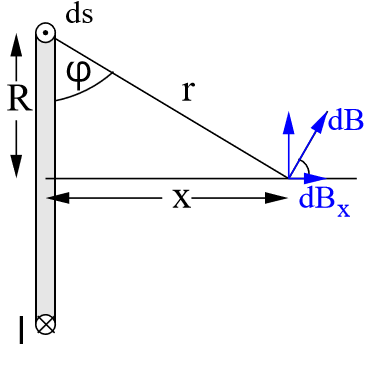
\includegraphics[width=5 cm , height=3.5 cm]{Abb1.png}
	\caption{Schematische Darstellung des Biot-Savartschen Gesetz \cite{1}.}
	\label{abb:1}
\end{figure}

Im Inneren für langgestreckten Spule (Solenoid) ist die magnetische Feldstärke $\vec{H}$
homogen und konstant während sie außerhalb inhomogen ist.
Mit der Spulenlänge $l$, der Windungszahl $n$ und den Strom $I$ lässt sich das
homogene Magnetfeld mit der Formel

\begin{equation}
  B = \mu_r \mu_0 \frac{n}{l} I
  \label{eq:3}
\end{equation}

darstellen.
Eine genauere Berechnung zur Magnetfeldstärke kann folgende Form verwendet werden

\begin{equation}
  B= \frac{\mu_0 n I R^2}{2} \cdot (\frac{x-x_1}{\sqrt{(x-x_1)^2 +R^2}} - \frac{x-x_2}{\sqrt{(x-x_2)^2 +R^2}})
  \label{eq:7}
\end{equation}

Die Herleitung dieser Gleichung wird aus \cite{2} entnommen.
Wird die langgestreckte Spule zu einem Kreis gebogen so wird die Spulenanordnung
als Torus bezeichnet. Die Besonderheit des Torus ist, dass außerhalb kein Magnetfeld
existiert und im Inneren das Magnetfeld homogen ist. Somit lässt sich die Gleichung(\ref{eq:3})
mit $l= 2\pi r_T$ zu

\begin{equation}
  B = \mu_r \mu_0 \frac{n}{2\pi r_T} I
  \label{eq:4}
\end{equation}

umschreiben. Dabei ist $r_T$ der Radius des Torus.
Ein anderes Verfahren zu Herrichtung eines homogenen Magnetfeldes ist die Helmholtz-Spule.
Zwei parallele Kreisspulen, die die gleiche Stromrichtung besitzen, erzeugen ein homogenes
Feld im Inneren der beiden Spulen. Eine Darstellung ist in Abbildung(\ref{abb:2}) zu sehen.

\begin{figure}[H]
  \centering
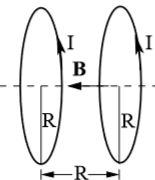
\includegraphics[width =5 cm, height = 3.5cm]{Abb2.png}
\caption{Schematische Darstellung der Helmholtz-Spule \cite{1}.}
\label{abb:2}
\end{figure}

Alternativ kann das Magnetfeld einer Helmholtz-Spule mit der folgenden Gleichung bestimmt
werden, die auch mit dem Biot-Savart-Gesetz bestimmt wurde. Mit dieser Gleichung wird das
Magnetfeld im Zentrum der Spule beschrieben, also an jeder Stelle der x-Achse.

\begin{equation}
  B_x = \frac{\mu_0 I}{2R} \left[ \frac{1}{\left(\left(\frac{x}{R}\right)^2 + \frac{x}{R} + \frac{5}{4} \right)^{\frac{3}{2}}}
  + \frac{1}{\left(\left(\frac{x}{R}\right)^2 - \frac{x}{R} + \frac{5}{4} \right)^{\frac{3}{2}}}\right]
  \label{eq:8}
\end{equation}

Diese Gleichung wird durch \cite{3} gegeben.
Ferromagnetische Materialien wie z.B. Eisen, Kobalt oder Nickel besitzen ohne ein äußeres Magnetfeld
ein permanentes magnetisches Moment. Magnetischen Momente richten sich in einzelnen Bereichen (Weißsche Bezirke)
parallel zu einander aus. Ohne äußeres Feld ist die Ausrichtung der Weißschen Bezirke statisch verteilt.
Mit einem äußeren Magnetfeld gibt es eine Richtungsänderung und zu einer Vergrößerung des Bezirks.
Dies wird solange ausgeführt bis alle magnetischen Momente mit der Ausrichtung vom Magnetfeld übereinstimmen.
Für ferromagnetische Materialien ist die relative Permeabilität $\mu_r$ sehr hoch, somit ist die Gültigkeit der
Gleichung (\ref{eq:1}) ungültig.
Die Hysteresekurve beschreibt diese Nicht-Linearität und ist in Abbildung (\ref{abb:3}) dargestellt.
\begin{figure}[H]
  \centering
  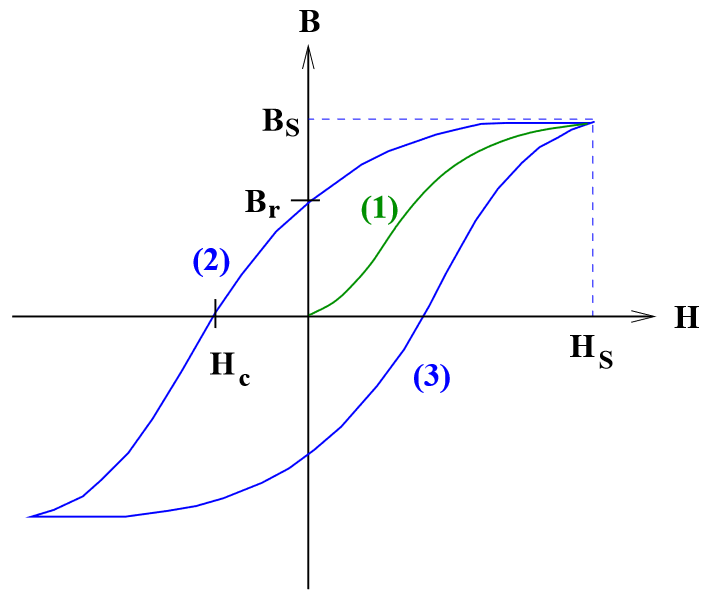
\includegraphics[width=10cm, height= 7cm]{Abb3.png}
  \caption{Schematische Darstellung einer Hysteresekurve \cite{1}.}
  \label{abb:3}
\end{figure}
In Abbildung (\ref{abb:3}) wird \textbf{1} als Neukurve bezeichnet.
Sie erreicht nach einiger Zeit ein Sättigungswert $B_s$. Beim Abschalten
des äußeren Magnetfeldes, bleibt noch beim Ferromagnet eine "Restmagnetisierung" die
als Remanenz bezeichnet wird. Die \textbf{2} beschreibt die Koerzitivkraft um die Remanenz auf null zu bekommen.
Durch Erhöhung des Gegenfeldes wird ebenfalls ein negativen Sättigungswert erreicht.
Die \textbf{3} zeigt den Kurvenverlauf durch Erhöhung des Magnetfeldes und sie ist symmetrisch zur Hysteresekurve.
Somit wird die relative Permeabilität $\mu_r$ eine Funktion zur Feldstärke $\vec{H}$.
Die Neukurve wird durch die differentielle Permeabilität $\mu_\text{diff}$ beschrieben und lautet
\begin{equation*}
  \mu_\text{diff} = \frac{dB}{\mu_0 \cdot dH}
  \label{eq:6}
\end{equation*}
